\documentclass[11pt, oneside]{article}   	% use "amsart" instead of "article" for AMSLaTeX format
\usepackage{geometry}                		% See geometry.pdf to learn the layout options. There are lots.
\geometry{letterpaper}                   		% ... or a4paper or a5paper or ... 
%\geometry{landscape}                		% Activate for for rotated page geometry
%\usepackage[parfill]{parskip}    		% Activate to begin paragraphs with an empty line rather than an indent
\usepackage{graphicx}				% Use pdf, png, jpg, or eps§ with pdflatex; use eps in DVI mode
								% TeX will automatically convert eps --> pdf in pdflatex		
\usepackage{amssymb}
\usepackage{amsmath}
\usepackage{parskip}
\usepackage{color}
\usepackage{hyperref}

\title{Triangle Inequality}
%\author{The Author}
%\section{}
%\subsection*{}
\date{}							% Activate to display a given date or no date

\graphicspath{{/Users/telliott_admin/Dropbox/Tex/png/}}
% \begin{center} 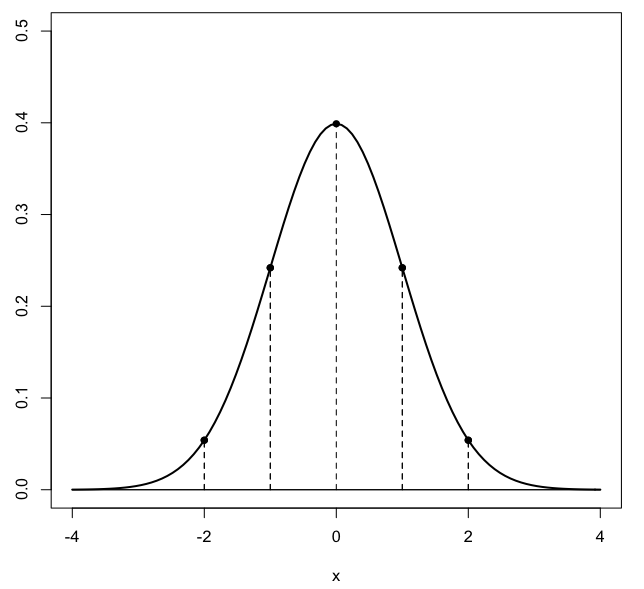
\includegraphics [scale=0.4] {gauss3.png} \end{center}
\begin{document}
\maketitle
\Large
Here we prove the theorem called the triangle inequality, which is used in numerous places in analysis.  It is a simple idea, obviously true, and yet restating the formal proof from memory can tie me up in knots.  

We first go through an informal proof by enumeration of cases before looking at the proof as presented in a famous textbook.

\subsection*{Absolute value}
The theorem involves the absolute value function, which is typeset as $f(x) = |x|$ and defined as follows:
\[
f(x) = |x| = 
\begin{cases}
\ \ 0, \ \ \ x = 0 \\
\ \ x, \ \ \ x > 0 \\
-x, \ \ \ x < 0
\end{cases}
\]
The definition can be simplified by combining the first two cases into one statement:  $|x| = x$ for $x \ge 0$.  But in what follows we will consider all three cases separately.

The triangle inequality says that for any two real numbers $a$ and $b$ 
\[  |a + b| \le |a| + |b| \]

In fact for many choices of $a$ and $b$, we have equality:
\[ |a + b| = |a| + |b|  \]

As an example, consider both $a > 0$ and $b > 0$.  By the definition of the absolute value function $a = |a|$ and $b = |b|$ so
\[ a + b = |a| + |b| \]
and since $a + b > 0$, $|a + b|$ is defined to be equal to $a + b$ so
\[ |a + b| = |a| + |b| \]

The same happens when either $a$ or $b$ is zero (or both), or when $a$ and $b$ are both negative.  In all these cases we have equality.  

The more challenging case is when $a > 0$ and $b < 0$.

\subsection*{Aside on geometry}
The triangle inequality is so named because a version from geometry says that when any two sides of a triangle are added together the resulting length is greater than the length of the third side.
\begin{center} 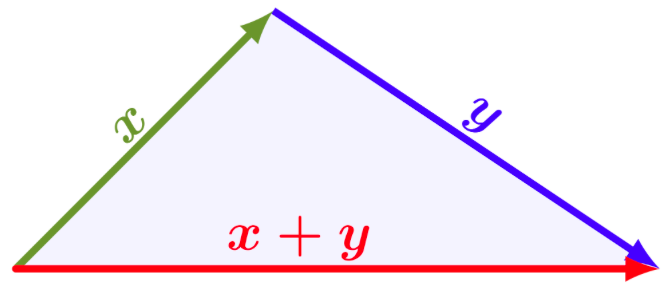
\includegraphics [scale=0.3] {triangle_inequality.png} \end{center}

The geometric version is pretty obvious.  Euclid teaches us that the shortest distance between any two points is a straight line (in this figure from the web, $\mathbf{x + y}$ refers to the \emph{vector sum} of $\mathbf{x}$ and $\mathbf{y}$).  The absolute value gives the length of a vector.

Equality is found for the limiting case when the triangle collapses.
\subsection*{Triangle equality:  real numbers}
However, we are interested here in the more general situation where $a$ and $b$ are real numbers, and thus, possibly negative. 

Going back to the statement of the theorem:
\[ |a + b| \le |a| + |b| \]

We will write equality (which is subsumed under the $\le$ sign) until we need to relax that condition.
\[ |a + b| = |a| + |b| \]
$\bullet$  $a = 0$ and $b = 0$

Write the left-hand side first, followed by the right-hand side.
\[ \text{lhs}: \ \ \  |a + b| = |0 + 0| = |0| = 0 \]
\[ \text{rhs}: \ \ \  |a| + |b| = |0| + |0| = 0 + 0 = 0 \]

$\bullet$  $a = 0$ and $b \ne 0$

\[ \text{lhs}: \ \ \  |a + b| = |0 + b| = |b| \]
\[ \text{rhs}: \ \ \  |a| + |b| = |0| + |b| = 0 + |b| = |b| \]

$\bullet$  $a > 0$ and $b > 0$

We did this one above.  The sum $a + b > 0$, so by the definition of the absolute value function

\[ \text{lhs}: \ \ \  |(a + b)| = (a + b) = a + b \]
\[ \text{rhs}: \ \ \  |a| + |b| = a + b \]

$\bullet$  $a < 0$ and $b < 0$

I find it easier to introduce positive values $m > 0$ and $n > 0$.  Define $a = -m$ and $b = -n$.

The sum $a + b = -m -n = -(m + n)  < 0$, so by the definition of the absolute value function

\[ \text{lhs}: \ \ \  |a + b| = |-(m+n)|  = m+n \]
\[ \text{rhs}: \ \ \  |a| + |b| = |-m| + |-n| = m+n \]

The last case is where $a$ and $b$ are of different sign.  This is where we need the inequality.

$\bullet$  $a > 0$ and $b < 0$

Consider $a > 0$ and $m > 0$ and define $b = -m$.
  
In terms of the number line, we imagine starting from the origin and moving right a distance $a$, then moving left a distance $m$.  

If $a \ge m$, the result is $a - m$ units to the right of the origin.  On the other hand, if  if $a < m$, the final position is $m - a$ units to the left of it.

$\circ$  If $a \ge m$ then $a + b = a - m \ge 0$.  From the definition of the absolute value (since $a - m \ge 0$):

\[ \text{lhs}: \ \ \  |a + b| =  |a - m| = a - m \]
\[ \text{rhs}: \ \ \  |a| + |b| = |a| + |-m| = a + m \]
But
\[  a - m < a + m \]
\textbf{Proof}:  start with $a \le a + 2m$, then add $-m$ to both sides.

$\circ$  If $a < m$ then $a + b = a - m < 0$ so $|a - m| = m - a$.

\[ \text{lhs}: \ \ \  |a + b| =  |a - m| = -(a - m) = m - a \]
\[ \text{rhs}: \ \ \  |a| + |b| = |a| + |-m| = a + m \]
and again, the first expression is $\le$ the second.  This completes the proof.
\subsection*{Apostol}
For a more formal approach (especially helpful for the case of different signs), we follow Apostol.  We prove a preliminary theorem first, which is another result frequently used in analysis.  

Consider an open interval whose endpoints are equidistant from a central point $p$, where the distance to the boundary is $a > 0$, and  $x$ is contained somewhere in the open interval $(p-a,p+a)$
\begin{center} 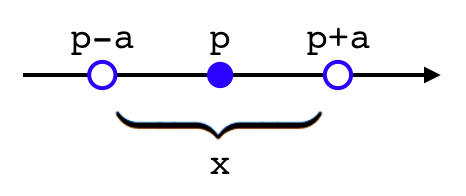
\includegraphics [scale=0.4] {neighborhood2.png} \end{center}

We can translate this picture to algebra as
\[ p - a < x < p + a \]
Adding $-p$ to each term
\[ -a < x - p < a \]
The preliminary theorem states that the above is true if and only if
\[ |x - p| < a  \]
We should read the last statement as saying that the distance between $x$ and $p$ is less than $a$.

\subsection*{continuity example}
As a motivating example, in the definition of \textbf{continuity} of a function $f(x)$ at a point $a$, we play the epsilon-delta game.  Choose an \emph{arbitrary} positive real number $\epsilon > 0$.  

Then we say, $f$ is continuous at $a$ if and only if we can find $\delta$ such that 
\[ |x - a| < \delta \Rightarrow |f(x) - f(a)| < \epsilon \]

The distance (or difference) between $x$ and $a$ is less than $\delta$ implies that the difference $|f(x) - f(a)|$ is less than $\epsilon$.

\begin{center} 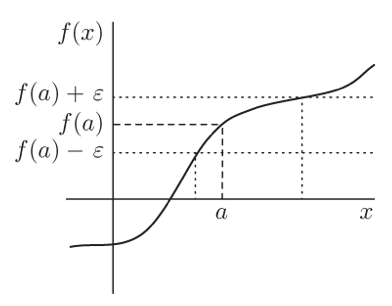
\includegraphics [scale=0.6] {continuity3.png} \end{center}
 
\subsection*{Informal proof}
\[ -a < x - p < a \Rightarrow  |x - p| < a  \]
may be proved informally by going exhaustively through the cases, as follows.

(1) If $x = p$ then $x - p = 0 < a$; 

(2) If $x > p$, then $x - p > 0$ and so 
\[ |x - p| = x - p \]
Then
\[ x - p < a \] 
implies 
\[ |x - p| = x - p < a \]

(3) If $x < p$ then $x - p < 0$ so
\[ |x - p| = -(x-p) = p - x \]
Then the first part of the assumption is
\[ -a < x - p \] 
Add $a + p - x$ to both sides
\[ p - x < a \]
which implies
\[ |x - p| = p - x < a \]
which proves the theorem.

You might think we're done, but I'd like to go through the more formal proof now.
\subsection*{Preliminary Theorem}
Taking the statements above
\[ |x - p| \le a \iff -a \le x - p \le a \]
and rewriting $x -p$ as just $x$ we obtain:  
\[ |x| \le a \iff -a \le x \le a \]
This is the version we will prove.

\subsection*{Proof}
Let $a$ be a constant real number $a \ge 0$ and the starting proposition is
\[ |x| \le a \]
Add the expression $-a - |x|$ to both sides to obtain
\[ -a \le - |x| \]

We need two more pieces.  First
\[ x \le |x| \]
If $x \ge 0$ then $x = |x|$ by definition, while if $x < 0$, then $x \le |x|$ since $|x|$ is always non-negative.  

Also
\[ - |x| \le x \]
If $x \ge 0$ then $x = |x|$ and clearly $-|x| \le |x|$.  Otherwise $x < 0$ and then $- |x| = x$.

We just combine all four inequalities:
\[ -a \le -|x| \le x \le |x| \le a \]
which simplifies to
\[ -a \le x \le a \]
This completes the forward proof.

To prove the converse, assume that
\[ x \le a \]
\[ - a \le x \]
Now if $x \ge 0$ we have $|x| = x$ so
\[ |x| = x \le a \]
On the other hand for $x < 0$, we start with the first part
\[ -a \le x \]
Add $a - x$ to both sides
\[ -x \le a \]
and since $x < 0$, $|x| = -x$ and we have 
\[ |x| =  -x \le a \]
In both cases we have \[ |x| \le a \]
and this completes the proof.

\subsection*{Triangle inequality}
Finally, change the notation of the previous theorem so we can reuse the variable $x$ in the next part:
\[ | \phi | \le a \iff -a \le \phi \le a \]

Now start by considering
\[ - |x| \le x \le |x| \]
If $x \ge 0$ clearly $-|x| \le 0$ so $-|x| \le x$ and since $x = |x|$ certainly $x \le |x|$.

On the other hand, if $x < 0$ (say $m > 0$ and $x = -m$), then
\[ - |-m| \le -m \le |-m| \]
\[ - m = -m \le m \]

Now add two such inequalities 
\[ - |x| \le x \le |x| \]
\[ - |y| \le y \le |y| \]
we obtain
\[ - \ [ \ |x| +  |y| \ ] \  \le x + y \le  |x| + |y|  \]
Recall the theorem we just proved with its new notation and focus on the right-hand side
\[  -a \le \phi \le a \]
Equate $a$ with $|x| + |y|$ and $\phi$ with $x + y$.  

Then the expression that we had above
\[ - \ [ \ |x| +  |y| \ ] \  \le x + y \le  |x| + |y|  \]
can be seen as equivalent to this expression in the theorem.  

Therefore, the left-hand expression must also be true, namely
\[ |\phi| \le a \]
\[ |x + y| \le  |x| +  |y| \]
This proves the triangle inequality.

\subsection*{corollary 1}
We will show that $|a - x| = |x - a|$.  Thinking of absolute value as another way of saying "distance", this is obviously true.

Here is a simple proof.  Start with
\[ |xy| = |x| \ |y| \]
Clearly this is true for both $x,y > 0$ and $x,y < 0$.  Suppose $x < 0$ with $m > 0$ and $y = - m$.  Then
\[ |xy| = |x (-m)| = |-xm| = xm = |x| \ |-m| = |x| \ |y| \]
Then given
\[ |xy| = |x| \ |y| \]
write
\[ |a - x| = |(-1)(x - a)| = |-1| \ |x - a| = |x - a| \]
\end{document}  